\section{Метрики для оценки генеративных моделей для трехмерных данных} \label{section:metrics-evaluation}

Имея метод для сравненения двух облаков точек (см гл. \ref{section:metrics-comparation}) можно перейти к созданию метрики, оценивающей потери алгоритма при воспроизведении форм исходных объектов.

Пусть у нас имеется набор облаков точек \(A\) и набор облаков точек \(B\). Требуется оценить насколько хорошо набор \(A\) воспроизводит форму исходных данных, представленных набором \(B\).

В работе \cite{lrgm-cloud} авторы предлагают ряд метрик для данной задачи. Опишем две из них: \textit{Покрытие (Coverage, COV)} и \textit{Минимальное сопоставимое расстояние (Minimum matching distance, MMD)}.


\subsection{COV метрика}

Для каждого объекта из набора \(A\), находим ближайшего соседа к нему из набора \(B\). Покрытие (COV метрика) считается как отношение количества объектов из набора \(B\), которые были сопоставлены объектам из набора \(A\), к числу всех объектов в наборе \(B\). Чем больше значение данной метрики, тем лучше набор \(A\) покрывает набор \(B\) \cite{lrgm-cloud}.

% that were matched
\subsection{MMD метрика}

Для вычисления данной метрики, мы каждому объекту из набора \(B\) сопоставляем ближайший к нему объект из набора \(A\) и затем высчитываем среднюю велечину расстояний. Чем меньше значение данной метрики, тем ближе набор \(A\) лежат к набору \(B\) \cite{lrgm-cloud}.


\subsection{Обсуждение}

COV метрика показывает насколько хорошо происходит покрытие набора \(B\) объектами из набора \(A\), а MMD метрика показывает близость (точность, fidelity) набора \(A\) к набору \(B\). 

Несложно придумать случай, когда COV метрика будет иметь большое значение и при это MMD также будет иметь большое значение. К примеру, пусть оба набора находятся внутри двух параллелипипедов, параллельных друг-другу и сильно удаленных друг от друга, причем объекты внутри парллелипиедов выстроены вдоль линий параллельности (см рис. \ref{fig:mmdcov1}). Тогда для каждого объекта из первого набора (красные элементы) ближайшим к нему из второго набора (зеленые элементы) будет объект лежащий напротив него (соединены пунктирной линией). То есть, будет выполнено полное покрытие зеленого набора красным набором. Но при этом, среднее значение MMD может быть сколь угодно большим (на рисунке она равняетя 80).

% УВЕЛИЧЕНИЕ ОБЪЕМА!! привести пример
% УВЕЛИЧЕНИЕ ОБЪЕМА!! картинка
\begin{figure}[h]
\centering
    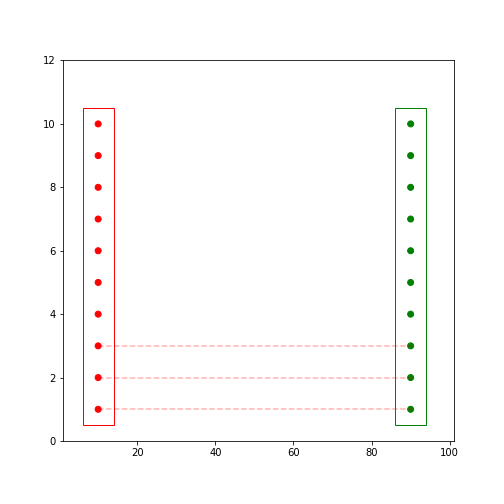
\includegraphics[width=0.6\textwidth]{images/MMD-COV-problem-1.png}
    \caption{Случай когда значения MMD и COV метрик велики}
    \label{fig:mmdcov1}
\end{figure}


Аналогично, можно придумать пример, когда одновременно COV метрика и MMD метрика будут иметь маленькие значения.
К примеру, объкты из набора $A$ сосредточены внутри некоторого шара $S_{A}$. И пусть почти все объекты набора $B$ также сосредоточены внутри шара $S_{B}$. Причем шары не пересекаются: $S_{A} \cap S_{B} = \emptyset$, но при этом лежат довольно близко. И пусть один из объектов $b$ из набора $B$ не лежащих внутри шара лежит на отрезке соединяющим центры шаров $S_{A}$ и $S_{B}$ (см рис. \ref{fig:mmdcov1}).
Тогда получится, что COV метрика будет крайне малой (покрывается только объект $b$), но значение метрики MMD будет мало, ибо расстояния между группами объектов небольшие (на рисунке оно не больше 10).

\begin{figure}[h]
\centering
    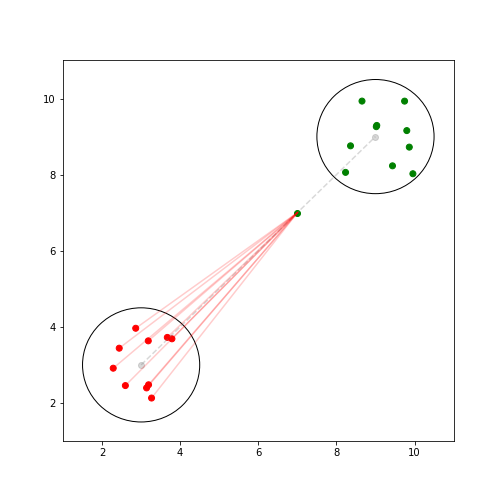
\includegraphics[width=0.6\textwidth]{images/MMD-COV-problem-2.png}
    \caption{Случай когда значения MMD и COV метрик малы}
    \label{fig:mmdcov2}
\end{figure}
% УВЕЛИЧЕНИЕ ОБЪЕМА!! картинка

В связи с этим, мы приходим к выводу о том, что COV и MMD метрики друг-друга отлично дополняют и их следует использовать в совокупности. И можно говорить о том, что набор сгенерированных объектов $A$ воспроизводит исходные формы объектов, представленные набором $B$, тогда, когда COV метрика велика, а MMD, наоборот, мала. Стоит отметить, что это является лишь необходимым, но не достаточным условием.